\documentclass[a4paper, 12pt, onecolumn, openright, oneside]{report}

\usepackage[utf8]{inputenc}
\usepackage[pdftex]{graphicx}
\usepackage{setspace}
\usepackage[T1]{fontenc}
\usepackage[francais]{babel}
\usepackage{color}
\usepackage{enumitem}
\usepackage{graphicx}
\usepackage{fancybox}
\usepackage{color}
\usepackage{geometry}
\usepackage{comment}
\usepackage{lipsum}
\usepackage[french]{minitoc}
\usepackage[nottoc]{tocbibind}
\usepackage[nottoc]{tocbibind}
\usepackage{fancyhdr} %pour definir les entêtes et pied de pages
\usepackage[Sonny]{fncychap} %style de chapitre
\usepackage{caption} %caption des images figure
\usepackage{epigraph} %citations%
\usepackage{lmodern}
\usepackage{dirtree}
% The following is a dummy icon command
\newcommand\myicon[1]{{\color{#1}\rule{2ex}{2ex}}}
% If you have actual icon images, use \includegraphics to include them
% If you are generating them, put in the appropriate code for them here
% now we make a command for a folder/file which inserts the icon and its label
% adjust this as needed. If you only have 2 icons, then you could create
% a \myfile and \myfolder command with the icon fixed.
\newcommand{\myfolder}[2]{\myicon{#1}\ {#2}}

\usepackage{pict2e} %shéma%
\pagestyle{fancy}
\fancyhead[C]{}
\fancyhead[L]{\leftmark}
\fancyhead[R]{}
\definecolor{rouge}{RGB}{255,112,119}
\definecolor{rouge-clair}{RGB}{255,163,168}
\definecolor{rouge-tres-clair}{RGB}{255,217,219}
\newcommand{\hr}{\rule{\linewidth}{0.5mm}}
\newcommand{\br}{\\[0.5cm]}
\renewcommand*{\familydefault}{\sfdefault}
%Numéro de sections dans la marge
\makeatletter
\def\@seccntformat #1{ %
\protect\makebox[0pt][r]{\csname the#1\endcsname \quad }}
\makeatother
\captionsetup{
font=footnotesize,
justification=raggedright,
singlelinecheck=false
}
\usepackage{xcolor}
\usepackage{adjustbox}

\newenvironment{colbox}[2]{%
    \begin{adjustbox}{minipage=[b]{380px},margin=1ex,bgcolor=#1,env=center}% or use `bgcolor={HTML}{#1}` if you want to force HTML colors
        \textbf{#2}\\
}{%
    \end{adjustbox}%
}

\begin{document}
  \begin{titlepage}
  \begin{minipage}[t]{7cm} %t = top%
    \flushleft 
\includegraphics[width = 5cm]{images/logo_istic.png}
  \end{minipage}
  \hfill
  \begin{minipage}[t]{7cm}
    \flushright 
\includegraphics[width = 5cm]{images/logo_capgemini.png}
  \end{minipage}
  \\[2cm]
  \begin{center}
    \hr\\[0.5cm]
    {\huge\textbf{Rapport de stage }}\\[0.4cm]
    {\large\textbf{Développeur sur le projet Geofibre}}\\[0.4cm]
    \hr\\[0.5cm]
    \textsc{Thibault Gauthier\footnote{Mise à jour le \today}}\\[0.4cm]
    Du 9 Mars au 28 Août 2015\\[2.5cm]
  \end{center}
  \begin{minipage}[t]{8cm} %t = top%
    \textbf{Tuteur en entreprise}\\
    \textsc{Monsieur Patrick VEILLON}\\[0.5cm]
    \textbf{Tuteur académique}\\
    \textsc{Monsieur François POULET}
  \end{minipage}
  \hfill
  \begin{minipage}[t]{8cm}
    \textbf{Entreprise d'accueil} \\
    \textsc{Capgemini}\\
    \textit{7 Rue Claude Chappe\\
    35510 Cesson-Sévigné}\\[0.5cm]
    \textbf{\'Etablissement de formation}\\
    \textsc{ISTIC\footnotemark}\\
    \textit{263 avenue du Général Leclerc\\
    35042 Rennes}\\[0.5cm]
    \textbf{Intitulé de la formation}\\
    \textsc{Master MIAGE\footnotemark}

  \end{minipage}
  %en dehors de l'env minipage
  \addtocounter{footnote}{-2} %3=n
  \stepcounter{footnote}\footnotetext{Unité de formation en informatique et électronique à l'université de Rennes 1}
  \stepcounter{footnote}\footnotetext{Méthodes informatiques appliquées à la gestion des entreprises}

\end{titlepage}

  %-------------------------------------------------------%
  \chapter*{Remerciements}
\begin{flushright}
Je tiens à remercier toutes les personnes qui ont contribué au bon déroulement de mon stage.
\\En premier lieu Monsieur \textsc{Patrick Veillon}, Madame \textsc{Anne-Sophie Lescop} ainsi que l'entreprise Capgemini
qui m'ont donné l'opportunité et accordé leur confiance pour réaliser mon stage de fin d'études.
\\Je remercie également Monsieur \textsc{Jérome le Dorze}, Monsieur \textsc{Gaëtan Vieau} et toute l'équipe du projet Geofibre (\textsc{Omar, Olivier, Xavier, Jalal, Gaël, Sébastien, Damien, Taher}) pour leur aide et leurs conseils tout au long du stage.
\\Pour finir, je tiens à manifester ma gratitude à Messieurs \textsc{Mickaël Foursov, Charles Queguiner, François Poulet et Didier Certain} ainsi qu'à l'ensemble des enseignants pour le bon déroulement de ces trois années du cursus MIAGE.
\end{flushright}

  %-------------------------------------------------------%
  \setcounter{secnumdepth}{1} %pas de numérotation des subsections
  \setcounter{tocdepth}{1}  %pas de numérotation des subsections
  \tableofcontents
  %-------------------------------------------------------%
  \chapter*{Introduction}
\addstarredchapter{Introduction}
La fin du master \textit{MIAGE} se concrétise par la réalisation d’un stage en entreprise d’une durée de 6 mois.
\\J’ai choisi de réaliser ce stage au sein de l’entreprise \textsc{Capgemini} du 9 mars au 21 août 2015,
dans le centre de services \textit{TMA OSS}\footnote{Tierce Maintenant Applicative des applications orientés réseau d'Orange} à Rennes.
\\Mon choix s’est porté sur ce stage pour plusieurs raisons.
 Tout d’abord la présentation du sujet m'a séduit, le projet \textit{Geofibre} m'a beaucoup plu.
 Ensuite, mes différentes expériences de stage ayant jusqu’alors été réalisées en
autonomie ou en binôme, je souhaitais intégrer une équipe de travail déjà en place.
\\Pour finir, je n'ai encore jamais travaillé dans une \textit{ESN}\footnote{Entreprise de services du numérique}, c'était l'occasion de se
faire une opinion.
\\\\
Dans un premier temps je présenterai le contexte du stage, l'entreprise d'accueil et le projet sur lequel j'ai travaillé.
Puis, dans un second temps je présenterai le stage en lui-même.

  %-------------------------------------------------------%
  \part{Contexte du stage}
  \chapter{La société Capgemini}
\subsection*{Introduction}
Capgemini est une ESN\footnote{Entreprise de services du numérique} multinationale spécialisée dans le génie logiciel.
\\Elle a été créee le 1er Octobre 1967 à Grenoble par Monsieur \textsc{Serge Kampf} et elle est actuellement dirigée par  Monsieur \textsc{Paul Hermelin}.\\
En France, elle est la première dans son domaine en terme de chiffre d'affaire. \'A l'internationale, elle figure parmi les cinq premiers.
\\Capgemini est notamment côtée en bourse au CAC40.
\\\\
\begin{figure}[h]
  \captionbox{Monsieur Serge KAMPF\label{fig:dummy}}{
    
\includegraphics[width=4cm]{images/sergekampf.png}
  }
  \captionbox{Monsieur Paul HERMELIN\label{fig:dummy}}{
    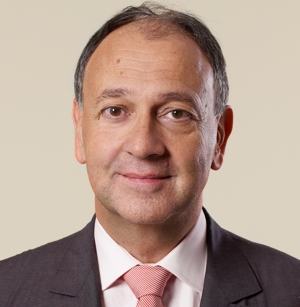
\includegraphics[width=4cm]{images/paulhermelin.png}
  }
  \captionbox{Logo de Capgemini\label{fig:dummy}}{
    
\includegraphics[width=5cm]{images/logo_capgemini.png}
  }
\end{figure}

\newpage
\section{Fiche d'identité}
\begin{description}
  \item[Raison sociale] : Capgemini
  \item[Année de création] : 1967
  \item[Fondateur] : Serge Kampf
  \item[Forme juridique] : Société anonyme à conseil d'administration
  \item[Siège social] : Paris
  \item[Directeur Général] : Paul Hermelin
  \item[Présence internationale] : 40 pays
  \item[Effectif en 2014] : 145 000
  \item[Chiffre d'affaire en 2014] : 10,6 milliards d'euros
\end{description}
\begin{figure}[h]
  \captionbox{Chiffre d'affaire par pays (2014)\label{fig:dummy}}{
    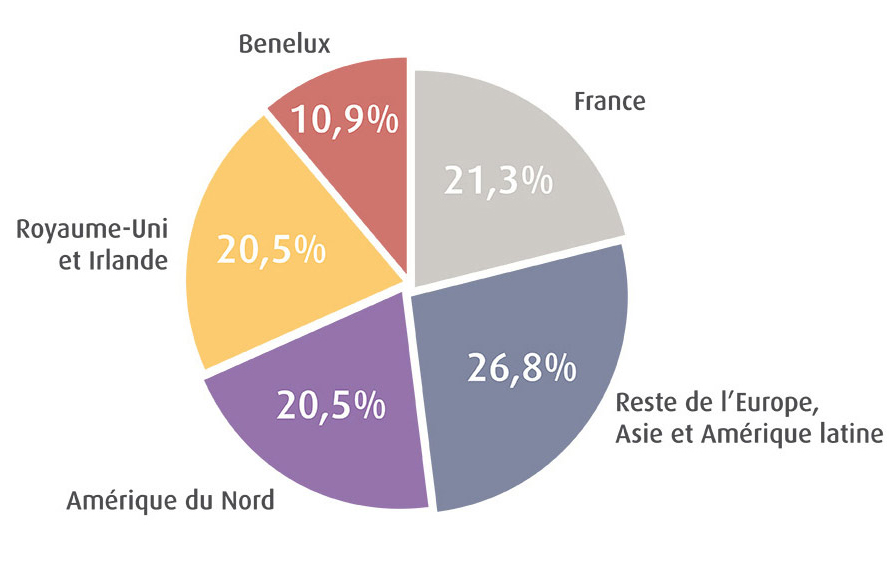
\includegraphics[width=15cm]{images/capays.png}
  }
\end{figure}
\newpage
\section{Métiers et activités}
\subsection{Secteurs d'activités}
Capgemini est spécialisé dans 6 secteurs d'activités :
\\
\begin{enumerate}
\item \textbf{Télécom, Média et \textit{Entertainment}}
\item \textbf{\'Energie, \textit{utilities} et chimie.}
\item \textbf{Industrie manufacturière et pharmaceutique}
\item \textbf{Services financiers}
\item \textbf{Grande consommation, distribution, transport et logistique}
\item \textbf{Services publics}\\
\end{enumerate}
\begin{figure}[h]
  \captionbox{Chiffre d'affaire par secteur (2014)\label{fig:dummy}}{
    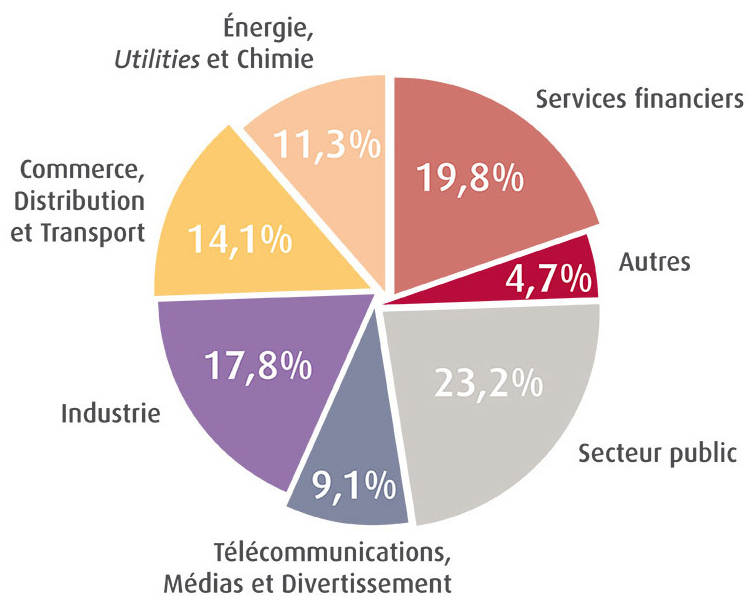
\includegraphics[width=12cm]{images/casecteur.png}
  }
\end{figure}
\newpage
\subsection{Métiers}
Capgemini travail dans 4 métiers principaux :
\\
\begin{enumerate}
\item \textbf{Le conseil en management (Capgemini Consulting)} a pour mission de contribuer, au travers d’actions telles que la transformation de l’activité ou la redéfinition de grandes fonctions, à l’amélioration des performances économiques des entreprises, grâce à une connaissance approfondie de leurs métiers et de leurs processus.
\item \textbf{L'intégration de systèmes et le développement d'applications} fait appel à la capacité de concevoir et d’intégrer des solutions, d’exploiter les innovations et de transformer l’environnement technologique.
\item \textbf{L’infogérance (Outsourcing Services - OS)} se concrétise par une prise en charge totale ou partielle de la gestion des ressources informatiques du client. Le Groupe a développé une gamme de services de gestion de systèmes informatiques, d’optimisation des processus métiers et de flexibilité des coûts de structures afin d’améliorer le rapport coût/performance.
\item \textbf{L'assistance technique et services de proximité (Sogeti)} ) sont implantés géographiquement au plus près des décideurs techniques locaux des grandes entreprises, visant à soutenir les capacités internes des directions informatiques en leur proposant dans des délais les plus brefs les meilleurs spécialistes.
\end{enumerate}
\begin{figure}[h]
  \captionbox{Chiffre d'affaire par metiers (2014)\label{fig:dummy}}{
    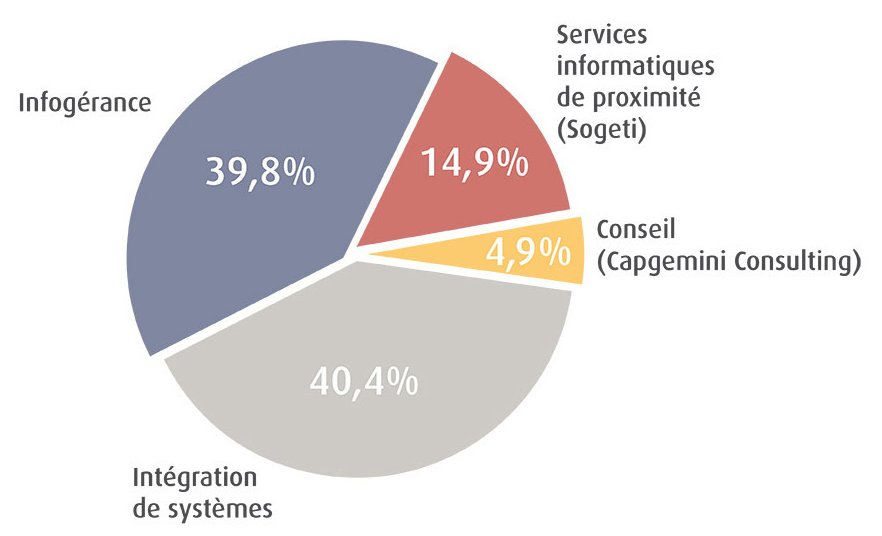
\includegraphics[width=13cm]{images/cametier.png}
  }
\end{figure}

  \chapter{Capgemini à Rennes}
\section{Fiche d'identité}
\begin{description}
  \item[Locaux] : Le Spiréa - Champs Blancs - Rennes
  \item[Année de construction] : 2012
  \item[Surface] : 9 850 m$^2$
  \item[Effectif en 2014] : 858
\end{description}
\begin{figure}[h]
  \captionbox{Le Spiréa à Rennes\label{fig:dummy}}{
    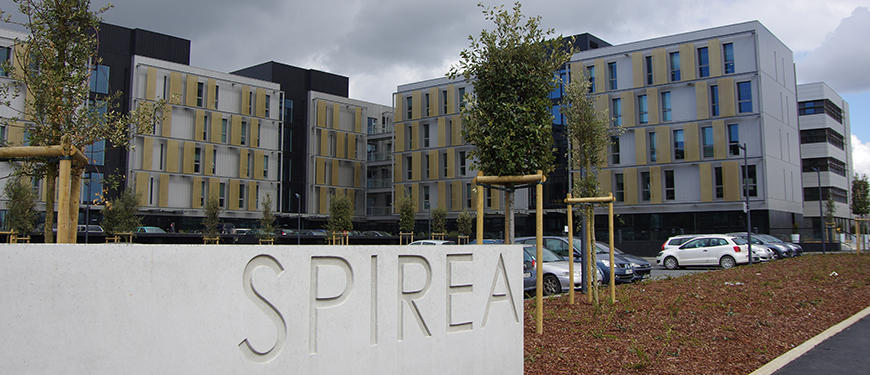
\includegraphics[width=15cm]{images/spirea.jpg}
  }
\end{figure}
\newpage
\section{Secteurs d'activités}
Le site de Rennes est divisé en 4 secteurs :
\begin{enumerate}
\item Aérospatiale et Défense
\item \textbf{ADM\footnote{Application Development and Maintenance} Center}
\item Services
\item Télécom et Média\\
\end{enumerate}

\begin{colbox}{{HTML}{C7FF99}}{}
  Mon stage c'est déroulé dans la division \textsc{ADM Center}.\\
  Dirigé par Monsieur \textsc{Jean-Louis Hammon}
  cette division s'occupe de la maintenance et de l'évolution d'application logiciel.
\end{colbox}

\section{Le centre de service TMA OSS}

La division ADM Center est subdivisé en plusieurs centre de services dont le service TMA OSS\footnote{Tierce Maintenance des Applications OSS d’Orange}.
Dirigé par Monsieur \textsc{Arnaud Bellina} ce centre s'occupe de la maintenance des applications orientée réseau pour le client Orange.
Il répond à diverses missions :

\begin{enumerate}
\item Développement d'évolutions
\item Soutien et maintenance
\item Audit et architecture
\item Assistance\\
\end{enumerate}

TMA OSS a 60 applications en activités et il est réparti sur 5 domaines différents :

\begin{enumerate}
\item \textbf{SIG\footnote{Système d’information géographique }}
\item Déploiement et interventions
\item Supervision QoS\footnote{Quality of Service}
\item RTG+\footnote{Ready-To-Go+} Supervision\\
\end{enumerate}

\section{Le domaine de compétence SIG}
\textsc{
Un système d’Information Géographique est un outil informatique permettant de représenter et d’analyser toutes les choses qui existent sur terre ainsi que tous les événements qui s’y produisent.
}\\\\
Les SIG offrent toutes les possibilités des bases de données (telles que requêtes et analyses statistiques) et ce, au travers d’une visualisation unique et d’analyse géographique propres aux cartes.
\\Ces capacités spécifiques font du SIG un outil unique, accessible à un public très large et s’adressant à une très grande variété d’applications.
Les enjeux majeurs auxquels nous avons à faire face aujourd’hui (environnement, démographie, santé publique…) ont tous un lien étroit avec la géographie.
De nombreux autres domaines tels que la recherche et le développement de nouveaux marchés, l’étude d’impact d’une construction, l’organisation du territoire, la gestion de réseaux, le suivi en temps réel de véhicules, la protection civile… sont aussi directement concernés par la puissance des SIG pour créer des cartes, pour intégrer tout type d’information, pour mieux visualiser les différents scénarios, pour mieux présenter les idées et pour mieux appréhender l’étendue des solutions possibles.
\\Les SIG sont utilisés par tous ; collectivités territoriales, secteur public, entreprise, écoles, administrations, états utilisent les Systèmes d’Informations Géographique (SIG). La création de cartes et l’analyse géographique ne sont pas des procédés nouveaux, mais les SIG procurent une plus grande vitesse et proposent des outils sans cesse innovant dans l’analyse, la compréhension et la résolution des problèmes.
\\L’avènement des SIG a également permis un accès à l’information à un public beaucoup plus large.
\\\\
Aujourd’hui, les SIG représentent un marché de plusieurs milliards d'euros dans le monde et emploient plusieurs centaines de milliers de personnes.
\begin{flushright}
\textit{source : Esri France}
\end{flushright}

  \chapter{Le projet Géofibre}
\section{Objet}
Le projet \textit{Geofibre} a pour objet de fournir une application de \textit{SIG} pour \textsc{Orange} dans le domaine du \textit{FTTH}\footnote{Fiber To The Home : C'est le réseau trés haut débit de fibre optique pour les clients résidentiels.}.\\
L'application se présente sous la forme d'une page Web permettant de gérer et concevoir des données descriptives du réseau \textit{FTTH} en France Métropolitaine (\textit{et depuis peu dans les départements d'Outre-Mer}), en temps réel avec plusieurs utilisateurs connectés simultanément.\\
Cette application est principalement destinée aux chargés d'affaire et sous-traitant \textit{FTTH}.\\
Elle a pour mission, par exemple, de faire évoluer le réseau en permettant la conception sur l'application pour ensuite l'imprimer et l'installer sur le terrain ou par exemple avoir une vision globale des installations sur une commune.\\
En matière de charge, elle comptabilise en 2015 jusqu'à \textbf{1150 utilisateurs simultanés}.\\
Techniquement \textit{Geofibre} est basé sur le progiciel \textit{ArcGIS} de l'éditeur \textsc{ESRI}.

\newpage
\section{Historique}
Le lancement du projet a eu lieu en 2010. Jusqu'en 2012 le projet s'est développé dans les locaux du client dans la ville de Lannion suivant la méthode de gestion de projets \textit{AGILE}.\\
Les employés de la société \textsc{Capgemini} étaient à cette époque présents dans les locaux du client pour travailler en tant qu'assistants techniques.
Par la suite le développement du projet s'est réalisé dans les locaux de \textsc{Capgemini}, au \textit{Spirea} à Rennes.\\\\
Depuis ses débuts \textit{Geofibre} a évolué de manière significative. \'A l'heure actuelle le projet est à sa 7ème version mineure(cf.\ref{versionning}) et des évolutions sont prévues, d'autant que le gouvernement Français souhaite développer la fibre optique sur l'ensemble du territoire Français.

\section{Illustration}
\begin{figure}[h]
	\captionbox{Capture d'écran du projet Geofibre\label{fig:dummy}}{
		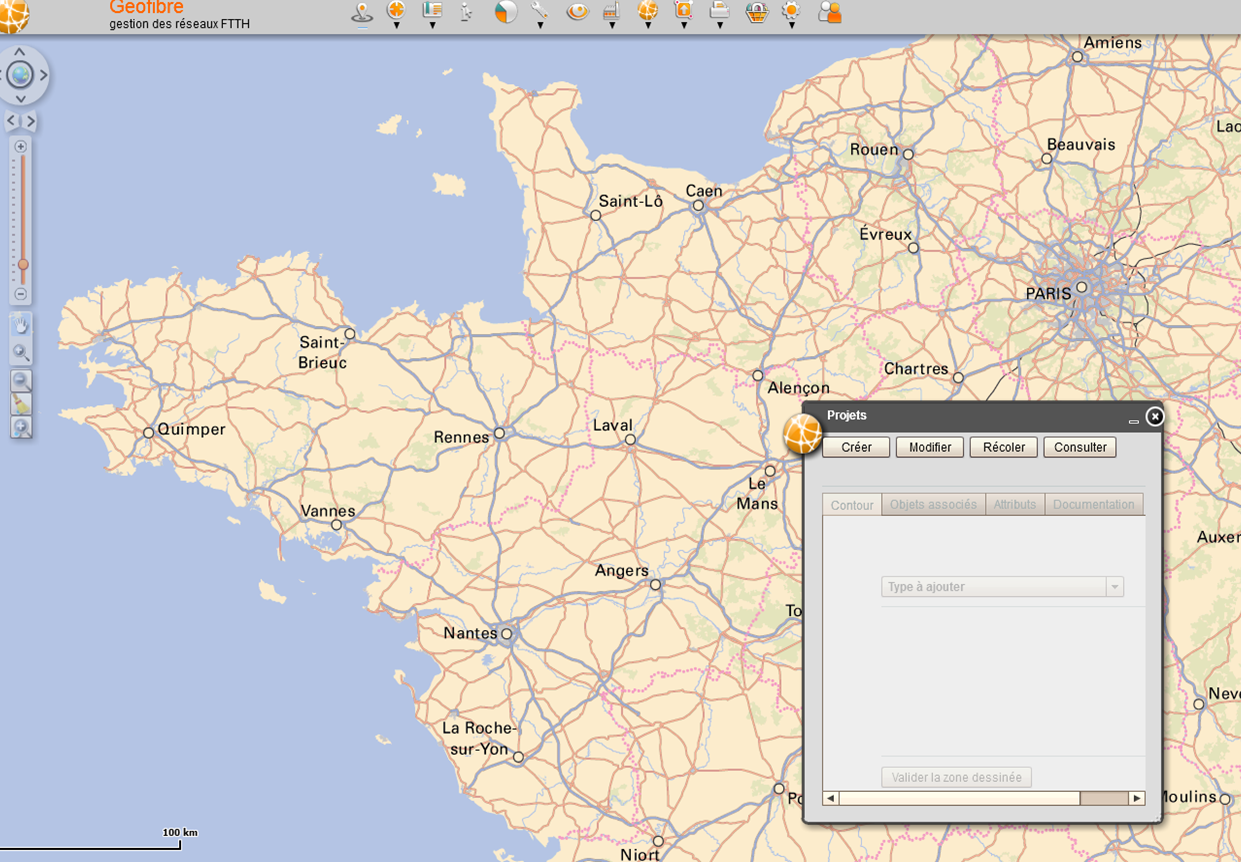
\includegraphics[width=16cm]{images/shotgeofibre.png}
	}
\end{figure}

  %-------------------------------------------------------%
  \part{Réalisation du stage}
  \chapter{Le Stage}
\section{Sujet}

Le sujet de stage est la participation au développement d'une évolution sur l'application \textit{Geofibre}.
Le client souhaiterait en effet intégrer de nouvelles fonctionnalités, notamment l'intégration des cartes des départements d'Outre-Mer au sein de l'application.
\\Cette version s'annonçant conséquente, l'équipe dirigeante a décidé de renforcer le groupe.

\section{Objectif}


L'objectif du stage est, dans un premier temps, de participer aux phases de développement jusqu'à la livraison pour l'évolution prévue sur l'application et dans un second temps de participer à la maintenance de l'application.

\chapter{Organisation de l'équipe}

L'équipe de travail est organisée de la façon suivante :\\

\begin{itemize}
  \item Le chef de groupe
  \item Le chef de projet
  \item L'équipe de développement
  \item Le responsable de test, c'est aussi le chef de projet.
  \item Le responsable du groupe, c'est un membre de l'équipe de développement.
  \item Le responsable du groupe 2, c'est un membre de l'équipe de développement.\\
\end{itemize}
Je suis intégré au sein de l'équipe de développement composée de 10 personnes (1 externe et 9 salariés).
\\Nous fonctionnons suivant la méthode \textit{LEAN}.

 \begin{colbox}{{HTML}{A3E8FF}}{La méthode LEAN\\ }
   \textbf{Objectif} : Améliorer de façon continue la performance en termes de qualité, coûts et délais de livraison.
   \\\textbf{Origine} : Apparue dans le seconde moitié du XXème siècle avec l'entreprise \textit{Toyota}. La production de voiture répond à une demande, ainsi les stocks sont quasi inexistants.
   \\\textbf{Principe} : Créer de la valeur ajoutée pour le client avec un minimum de gaspillage et en livrant un maximum de qualité.
   \\\textbf{En tant que développeur} : Des indicateurs de qualité de code à améliorer au fil des versions, des délais de livraison du service fini à respecter.
 \end{colbox}

 Chaque jour à 9h30 nous avons une réunion (\textit{Daily meeting}) où chaque membre de l'équipe, tour par tour, décrit son humeur de la veille, les tâches qu'il a réalisées, les problèmes éventuels à signaler et ce qu'il prévoit de faire au fil de la journée.
 \\ C'est une méthode qui permet de savoir où en est le projet, et plus particuliérement chaque membre de l'équipe. \\Cette méthode permet aussi de chercher les solutions ensemble aux problèmes et affecter plus de personnes sur une tâche bloquante dans la limite du possible.
\\La communication et la transparence sur le travail réalisé font que les problèmes ne restent pas longtemps sans solutions.
\\De plus, l'aménagement de l'\textit{Open-Space} permet de demander de l'aide rapidement aux collègues de travail; ça permet de ne pas rester bloqué sur une tâche ou se désorienter.
\\Le chef de projet écrit des fichiers de suivi d'avancement des tâches pour chaque phase du cycle du projet. Aux développeurs de le remplir en indiquant le temps passé sur chaque tâche réalisée et d'évaluer le \textit{RAF\footnote{le Reste à Faire}}. De cette manière le chef de projet et le chef de groupe peuvent planifier et piloter avec des risques moindres la suite du projet.

\chapter{Environnement technique}
\section{Architecture technique}
L'architecture technique repose sur des machines virtuelles (excepté la textit{BDD}).
Voici la liste des infrastructures présentes :
\begin{description}
\item[Serveur WAS] C'est le serveur qui délivre l'application à l'utilisateur. En effet, l'utilisateur s'y connecte via le \textit{GASSI}\footnote{Gestionnaire d'Accès Sécurisé interne au Système d'Information} du client avec le protocole \textit{HTTPS}\footnote{Hypertext Transfer Protocol Securised} ou via un \textit{VPN}\footnote{Virtual Private Network} avec le protocole \textit{SSL}\footnote{Secure Sockets Layer}.
\\Il fonctionne sur une machine Linux avec le serveur d'applications \textit{JOnAS}\footnote{Java Open Application Server}.
\item[Serveur ArcGIS] Basé sur le progiciel \textit{ArcGIS} de l'éditeur \textit{ESRI}, il permet de traiter les données \textit{SIG} (calcul de projection, géométries ...). Il délivre les informations récoltées et traitées à partir de la base de données au serveur \textit{WAS} sur la base d'une architecture \textit{REST}\footnote{REpresentional State Transfer}; Il communique aussi avec des interfaces externes, par exemple avec l'application \textit{Sigeo} (développé par \textsc{Capgemini}) pour récupérer les \textit{tuiles}\footnote{Images de fond de plan et images du cadastre}.
\item[Serveur d'impression] En raison de la charge induite par la génération des documents (\textit{PDF}) destinés à l'impression de fond de plan (certains aux formats A0), des serveurs sont dédiés à cette tâche. Il fonctionne eux aussi avec le progiciel \textit{ArcGIS}.
\item[Serveur SGBD] Le serveur de base de données est \textit{PostGreSQL} et permet de gérer l'accès et le stockage des données.\\
\end{description}

\'Etant donné la charge sur l'application, il existe plusieurs instances de serveurs et la communication d'un serveur à un autre se fait via des répartiteurs de charges qui vont requêter le bon serveur au bon moment afin d'équilibrer la charge de travail entre les différents serveurs. De ce fait il y a, en plateforme de production :\\

\begin{itemize}
	\item 3 serveurs WAS
	\item 8 serveurs ArcGIS pour la France Métropolitaine et 2 pour les DOM
	\item 1 serveur de base de données
	\item 4 serveurs d'impressions\\
\end{itemize}
\section{Outils et technologies}
\subsection{Adobe FlashBuilder}
C'est un environnement de développement d'applications basé sur le langage \textit{Actionscript} et le \textit{framework Flex Open Source}.
 \\On l'utilise pour développer et débuguer l'application \textit{front-office} qui sera placée sur le serveur WAS.
\subsection{Mozilla Firefox}
C'est un navigateur web.
 Il permet d'accéder à l'application via l'\textit{URL} du serveur qui délivre une page \textit{HTML} avec l'application \textit{front-office} embarquée dans un objet \textit{Flash}.
 \\Aussi on utilise le plugiciel \textit{Firebug} qui permet de voir les requêtes \textit{HTTP} envoyées et reçues par l'application,
 ça permet de débuguer les communications avec le serveur.
\subsection{Eclipse} \textit{Eclipse} est un environnement de développement basé sur le langage \textit{Java}. Nous utilisons un environnement \textit{JEE} afin de développer et débuguer le \textit{back-office} qui intègre le \textit{SDK ArcGIS} et qui permet de faire
 les tâches relatives au \textit{SIG}.
\subsection{Qgis Desktop} C'est un logiciel qui permet de visualiser des données \textit{SIG}. On l'utilise pour vérifier si des données sont bien représentées dans les phases de tests ou pour construire des jeux de données.
\subsection{PgAdmin} C'est une interface d'administration à la base de données \textit{PostgreSQL} utilisé par le projet.
\subsection{shell Linux} Afin d'accéder aux serveurs \textit{WAS, ArcGIS ou SGBD} via \textit{ssh} et lancer différents scripts sur les machines (par exemple il y a un script pour la copie de données d'une commune à une autre).

\chapter{Configuration du projet}
\section{Identification des versions}
\label{versionning}
Les versions sont marquées par des labels qui doivent permettre d'identifier de façon non équivoque toutes les évolutions successives des composants pour pouvoir retrouver et extraire de la base d'archives toute version livrée au client ou livrée pendant les phases d'intégration ou de la validation interne.
\\\\
On distingue deux types de versions :
\begin{description}
	\item[Version majeure] : c'est une version complète du logiciel, c'est-à-dire qu'elle contient l'ensemble des composants du système
	\item[Version mineure] : c'est une version partielle du logiciel, c'est-à-dire qu'elle ne contient qu'un sous-ensemble des composants du système, qui constitue un delta par rapport à la version précédente
	(qui peut être une version majeure ou mineure) ; c'est en général le résultat d'une correction ou d'une évolution mineure.
\end{description}
Les labels de version sont structurés de telle sorte que cette dépendance entre versions soit mise en évidence.
\\La composition d'un label de version est de la forme \textsc{GxxRyyCzz}.
\\Dans ce sigle on retrouve :
\begin{description}
	\item[Révision] : une révision est attachée à un composant. \'A chaque fois qu'un utilisateur archive une nouvelle version d'un composant, l'outil de gestion de configuration créée une nouvelle révision de ce composant.
	\item[Version et labels] : une version permet d'identifier un ensemble cohérent de composants d'une application. L'identifiant de version est sous contrôle complet de l'équipe de projet. Par exemple la première version est la G1R0C0, puis les suivantes seront les
	G1R1C0 puis la G2R0C0.
	\item[Tronc et branches] : le \textit{tronc} supporte les versions principales. En cas de travaux parallèles sur plusieurs versions (par exemple la correction d'une anomalie sur une version n-1 et développement de la version n), on crée une branche qui va permettre de modifier une version déjà livrée.
	\\
\end{description}
\textbf{Exemple} : La branche G1R0 contient les versions correctives G1R0C1 et G1R0C2 qui intègrent des correctifs d'anomalies identifiées sur la version G1R0C0 préalablement livrée.
\setlength{\unitlength}{1.3cm}

\begin{picture}(5,5)
	%texte
	\put(-2,4.4){Tronc}
	\put(-2,2.4){Branche G1R0}
	%traits haut
	\put(2.5,4.4){\vector(1,0){1.5}}
	\put(6.5,4.4){\vector(1,0){1.5}}
	\put(10.5,4.4){\vector(1,0){1.5}}
	%oblique
	\put(1.5,4){\vector(0.3,-1){0.5}}
	%traits bas
	\put(4.5,2.4){\vector(1,0){1.5}}
	\put(0,4){\framebox(2.5,0.8)[c]{G1R0C0}}
	\put(4,4){\framebox(2.5,0.8)[c]{G1R1C0}}
	\put(8,4){\framebox(2.5,0.8)[c]{G2R0C0}}
	\put(2,2){\framebox(2.5,0.8)[c]{G1R0C1}}
	\put(6,2){\framebox(2.5,0.8)[c]{G1R0C2}}
\end{picture}
\begin{colbox}{{HTML}{C7FF99}}{}
Durant mon stage j'ai participé à l'intégration de la 6ème version (G1R6C0) et au développement et à l'intégration de la 7ème version (G1R7C0).
\end{colbox}

\newpage

\section{Organisation des environnements de travail}

Le \textbf{référenciel} (\textit{Repository}) contient l'ensemble des révisions de chaque composant ainsi que les liens entre composants permettant d'identifier les versions successives de chaque application.
\\\\
Les \textbf{espaces de travail} (\textit{Workspaces}) sont les espaces utilisés pour développer, intégrer, valider et livrer chaque application.
\\
\begin{picture}(0,1)
	%Referenciel
	\put(0,-2){Référenciel}
	\put(0.7,-1.5){\oval(2,2)[t]}
	\put(-0.3,-2.5){\line(0,1){1}}
	\put(1.7,-2.5){\line(0,1){1}}
	\put(0.7,-2.5){\oval(2,2)[b]}
	%fleches
	\put(1.7,-1.5){\vector(1,0){6}}
	\put(2.6,-1.4){Extraction des composants}

	\put(7.7,-2.5){\vector(-1,0){6}}
	\put(2.6,-2.4){Archivage des composants}
	%espaces de travail x+8
	\put(7.8,-2){Espaces de travail}
	\put(8.2,-2.6){Composants}
	\put(8.7,-1.5){\oval(2,2)[t]}
	\put(7.7,-2.5){\line(0,1){1}}
	\put(9.7,-2.5){\line(0,1){1}}
	\put(8.7,-2.5){\oval(2,2)[b]}
	%+0.3
	\put(9,-1.5){\oval(2,2)[t]}
	\put(8,-2.5){\line(0,1){1}}
	\put(10,-2.5){\line(0,1){1}}
	\put(9,-2.5){\oval(2,2)[b]}

	\put(9.3,-1.5){\oval(2,2)[t]}
	\put(8.3,-2.5){\line(0,1){1}}
	\put(10.3,-2.5){\line(0,1){1}}
	\put(9.3,-2.5){\oval(2,2)[b]}

\end{picture}
\\[6cm]
Quand l'activité le justifie, il est possible de devoir travailler simultanément sur plusieurs versions, en général :
\begin{itemize}
	\item Une version en \textbf{développement}
	\item Une version en \textbf{maintenance}\\
\end{itemize}
Il faut donc prévoir autant d'espaces de travail disponibles et ceci pour les différentes phases du cycle de développement :
\begin{itemize}
	\item Développement et tests unitaires
	\item Intégration et validation
	\item Livraison (effectuée sur la plate-forme de qualification)\\
\end{itemize}
\newpage
\textit{Geofibre} est versionné avec \textit{SVN}\footnote{Subversion}, voici la hiérarchie des projets du \textit{repository} :\\

\dirtree{%
.1 \myfolder{red}{Trunk }.
.2 \myfolder{black}{gfi-front \textit{frontoffice}}.
.3 \myfolder{black}{5 projets}.
.2 \myfolder{black}{gfi-back \textit{backoffice}}.
.3 \myfolder{black}{7 projets}.
.2 \myfolder{black}{gfi-bdd \textit{base de données}}.
.3 \myfolder{black}{3 projets}.
.2 \myfolder{black}{gfi-expl \textit{exploitation}}.
.3 \myfolder{black}{9 projets}.
}


\chapter{\'Evolutions et mise en place}
\section{Version G1R6}

La version applicative G1R6 de \textit{Geofibre} doit permettre la prise en compte des DOMs. Pour cela des instances spécifiques sont mises en place  pour les différents départements (Réunion, Martinique, Guadeloupe et Guyane).
La mise à disposition de \textit{Geofibre} dans les DOMs doit être équivalente vue de l’utilisateur à la version métropole.
\\Les données dans les DOMs seront gérées dans le système de projection locale. Il n’y aura pas, comme en métropole (Lambert II étendu vers Lambert 93), de reprojection vers le système local ou d’export de données vers un autre système.\\

\begin{tabular}{|l|c|r|}
  \hline
    Zone & Système géodesique & Projection \\
  \hline
  France métropolitaine & RGF93 & Lambert 93 \\
  Guadeloupe & WGS84 & UTM Nord fuseau 20 \\
  Martinique & WGS84 & UTM Nord fuseau 20 \\
  Guyane & RGFG95 & UTM Nord fuseau 22 \\
  Réunion & RGR92 & UTM Sud fuseau 40 \\
  \hline
\end{tabular}\\\\

Malgré le fait que les serveurs soient hébergés en métropole, les horaires de création ou modification des objets stockés en base DOMs seront renseignés en heure locale.

\section{Version G1R7}
Cette version est essentiellement  fonctionnelle et dédiée à la prise en compte des paliers \textit{RIP}\footnote{Les réseaux d’initiative publique} et \textit{DSP}\footnote{Délégation de Service Public}.

\section{Cycle de développement en V}
Le projet fonctionne en cycle en V, suivant ce schéma :\\
\noindent%
\begin{minipage}{\linewidth}% to keep image and caption on one page
\makebox[\linewidth]{%        to center the image
  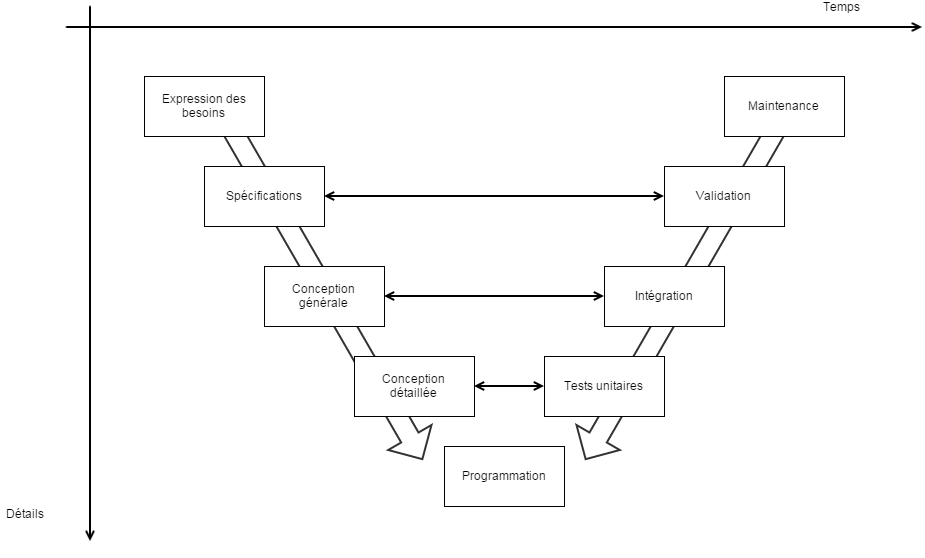
\includegraphics[keepaspectratio=true,scale=0.8]{images/cycle_en_v.png}}
\captionof{figure}{Cycle de développement en V}\label{visina8}%      only if needed
\end{minipage}
\newpage
\section{Planification}
Voici le planning qui représente la répartition des tâches durant mon stage :\\\\
\noindent%
\begin{minipage}{\linewidth}% to keep image and caption on one page
\makebox[\linewidth]{%        to center the image
  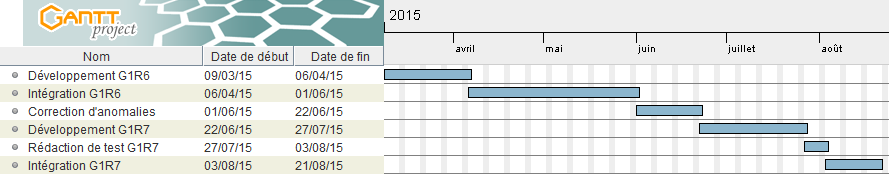
\includegraphics[keepaspectratio=true,scale=0.8]{images/gant.png}}
\captionof{figure}{Planning des tâches réalisées}\label{visina8}%      only if needed
\end{minipage}

En \textbf{annexe \ref{travauxreal}}, vous pouvez trouver le \textit{Carnet de bord des travaux réalisés par semaine}.
\chapter{Travail réalisé}
Je suis arrivé sur le projet lorsque la version G1R6 était à la fin de la phase de programmation. J'ai donc participé un peu à la phase de programmation puis à la phase d'intégration et de maintenance.
\\J'ai pu commencer la version G1R7 de la rédaction des spécifications jusqu'à l'intégration.
\section{Développement}
\subsection{Version G1R6}
On m'a rapidement permis de développer sur le projet. La première tâche consistait à externaliser des paramètres de configuration concernant le zoom, la projection et la mini-carte qui se trouve "en dur" dans l'application.
\\Cette première tâche de développement m'a permis de mieux comprendre le fonctionnement du projet. J'ai effectivement dû modifier trois sections de l'application :\\
\begin{itemize}
\item La base de données (gfi-bdd). En insérant de nouvelles données dans la table de configuration.
\item Le back-office (gfi-back). En faisant le mapping\footnote{Association des données en base à des objets en programmation} des données.
\item Le front-office (gfi-front). En supprimant les données de configuration "en dur" dans le programme et en envoyant les bonnes commandes au serveur pour récupérer les paramètres de configurations présentes en base de données.\\
\end{itemize}
Au départ j'ai rencontré beaucoup de problèmes, je n'étais pas sûr de ce que je faisais alors je posais beaucoup de questions à mes collègues de travail.
\\ Ensuite j'ai eu en charge de vérifier si le paramètre de projection était bien transmis aux  \textit{Toolboxs\footnote{Les toolboxs sont des \textit{servlets Java}, ce sont des extensions des fonctions du serveur de base.}} (gfi-back) et si elles étaient bien aiguillées en fonction de ce paramètre de projection.
Pour cela j'ai dû vérifier les requêtes envoyées par le client lors de l'appel de la toolbox et vérifier dans le back-office si le paramètre était bien transmis et vers la bonne servlet en débuggant le serveur \textit{Java}.

\subsection{Version G1R7}
Lors de la phase de développement de la version G1R7 j'avais beaucoup' plus d'expérience sur le projet, j'ai pu avancer sans beaucoup de problèmes et j'avais déjà des idées sur l'implémentation à adopter pour ce que je devais faire.
\\En effet je me suis occupé du widget \textit{Publication de Schéma Directeur} (gfi-front, gfi-back, gfi-data) où j'ai ajouté le champ opérateur au niveau de la base de données et de l'\textit{IHM}. Puis j'ai modifié les commandes de sélections, d'extraction et d'impression pour qu'elles se réalisent avec un filtrage sur le champ opérateur.
\\\\
\noindent%
\begin{minipage}{\linewidth}% to keep image and caption on one page
\makebox[\linewidth]{%        to center the image
  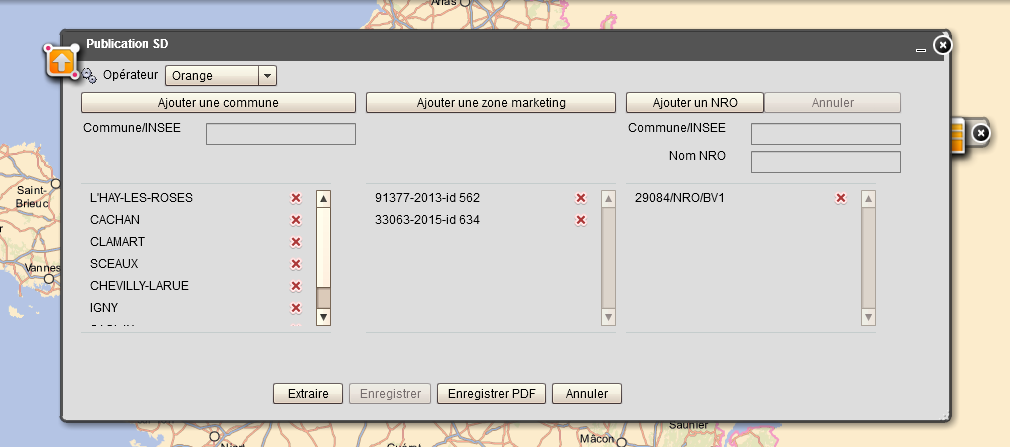
\includegraphics[keepaspectratio=true,scale=0.5]{images/publicationSD.png}}
\captionof{figure}{Widget publication SD}\label{visina8}%      only if needed
\end{minipage}\\

Je me suis ensuite occupé du \textit{programme de copie de données} (gfi-expl), qui permet de copier des données \textit{FTTH} d'une commune à une autre.
\\J'ai ajouté une contrainte liée à la configuration des \textit{RIP} : si la commune d'export n'a pas de configuration \textit{RIP} alors elle prend pour valeur la configuration \textit{RIP} de la table source.

\section{Intégration}
La phase d'intégration permet de tester le bon fonctionnement des développements réalisés.
\\\\
Le chef de projet commence par attribuer les tests aux différents développeurs avec le logiciel \textit{HP QC}; ensuite il nous suffit de filtrer les tests pour exécuter ceux qui nous sont attribués.
\\Le passage d'un test se déroule de la manière suivante :
\begin{enumerate}
\item on exécute les tests par priorité (P1,P2 puis P3).
\item on passe le test en cours d'exécution pas par pas.
\item si une étape se déroule comme prévu (\textit{result obtained} = \textit{result excepted}) on met l'étape à l'état \textit{passed} et on passe à la suivante.
\item si une étape échoue, on met l'étape à l'état \textit{failed} et si ce n'est pas déjà fait, on créer une anomalie (\textit{defect}). On y décrit l'anomalie détectée ainsi que la version d'intégration.
\item si on est bloqué sur une étape, par exemple s'il manque des données on met l'étape à l'état \textit{bloqued} et on
 met le test de côté pour le continuer lorsque l'étape sera débloquée.\\
 \end{enumerate}

 Une fois la phase de tests terminée, si des anomalies sont détectées le chef de projet dispatche les corrections et on passe à une nouvelle version d'intégration jusqu'à ce qu'il n'y ait plus aucune anomalie. C'est un système de vague, ainsi pour la version G1R6 il y a eu 6 vagues et pour la version G1R7 j'ai terminé mon stage pendant que nous étions à la 2ème vague d'intégration.

\section{Corrections d'anomalies}
Une fois l'intégration et la livraison terminée pour la version G1R6, les responsables des groupes travaillent avec le client sur l'élaboration des spécifications de la version G1R7.
\\Pendant ce temps je me suis occupé de corriger des anomalies en garantie que le client a détectées et a choisi de faire corriger pour la version G1R7, ce sont les \textit{anomalies éligibles à la version G1R7}.
\\Sous le logiciel \textit{HP QC} les anomalies sont répertoriées avec leurs détails et un descriptif écrit par le client.
\\Il s'agit donc de reproduire l'anomalie sur une version G1R6 de \textit{Geofibre} et de la corriger. Une fois corrigée, le code est commité sur la branche \textit{G1R7} et une synthèse est écrite par le correcteur.
\\\\
\noindent%
\begin{minipage}{\linewidth}% to keep image and caption on one page
\makebox[\linewidth]{%        to center the image
  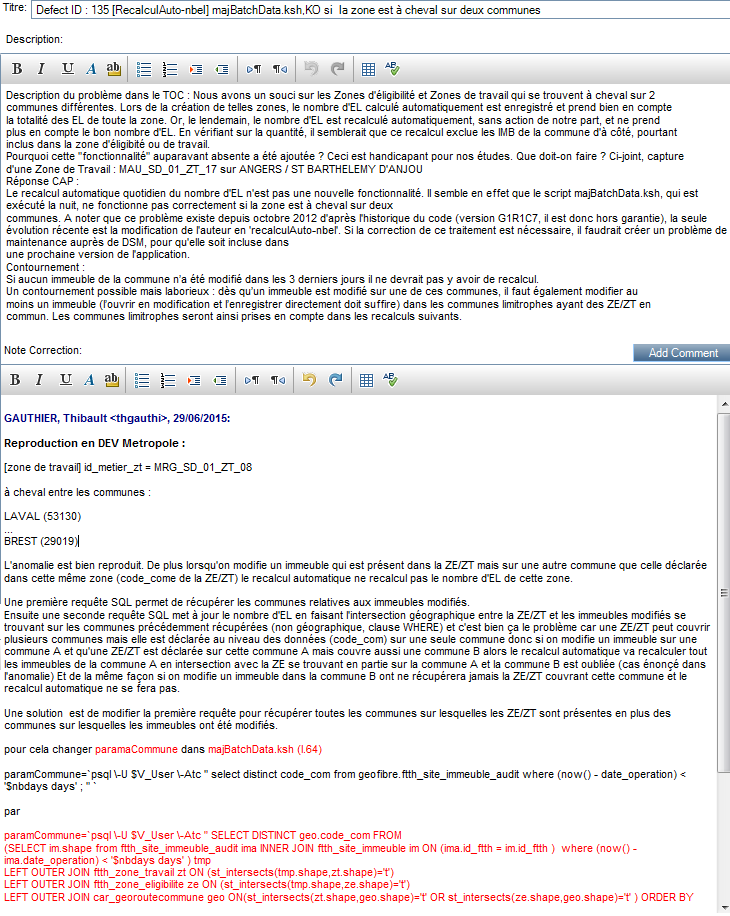
\includegraphics[keepaspectratio=true,scale=1]{images/exano.png}}
\captionof{figure}{Exemple de la synthèse de correction d'une anomalie}\label{visina8}%      only if needed
\end{minipage}\\
\section{Bilan du travail réalisé}

J'ai beaucoup appris sur l'organisation d'une équipe et d'un projet. Les différentes étapes du cycle en V sont bien exécutées selon les règles de l'entreprise \textsc{Capgemini}.
\\\\De plus, c'est un projet déjà bien en place, de ce fait je n'ai pas beaucoup développé, mais plutôt fait de la lecture, compréhension et modification de code.
\\\\Durant ces 6 mois de stage j'ai pris le temps de comprendre et de m'adapter au code de l'application. Je me suis rendu compte de l'importance d'une bonne architecture logicielle à la base d'un projet. Par exemple, lorsqu'on devait gérer un nouveau champ au niveau du front-office l'architecture qui n'avait pas bougé depuis plus de 3 ans le permettais. Je me suis aussi rendu compte que les commentaires étaient importants dans le code.

  %-------------------------------------------------------%
  \chapter*{Résumé}
\addstarredchapter{Résumé} 

  \chapter*{Abstract}
\addstarredchapter{Abstract}

My \textit{Master 2 MIAGE} internship was carried out within the company \textsc{Capgemini} at Rennes during six month.
\\\\
Within the service \textit{TMA OSS} I participated in the development and maintenance on \textit{Geofibre} application.
This application of \textit{GIS} enables business managers, via a \textit{web GUI}, to manage and develop the domestic \textit{FTTH} network in metropolitan France.
\\\\
My role was to provide the support to the development team for the integration of a new version of the application
to manage the \textit{FTTH} network of Overseas Departments ( French Guyana, Guadeloupe , Martinique and Réunion) .
Then, during the specification phase of the next release I spent to correct severals defects noted by the client.
Finally I participated in the development and integration of the latest version of the application that makes the management of new operators data.

  %-------------------------------------------------------%
  \chapter*{Conclusion}
\addstarredchapter{Conclusion}

Pour commencer le projet Geofibre est très intéressant de bout en bout et pour commencer m'a permis de découvrir le monde du SIG et du FTTH.
\\Techniquement j'ai pu découvrir le langage ActionScript et le framework Flex avec la programmation évenementiel même si c'est une technologie de moins en moins utilisée.
 \\ J'ai aussi pu découvrir le fonctionnement et l'utilité du progiciel ArcGIS.
 \\Aussi j'ai appris beaucoup de petites techniques de développement et de débuguage, notamment sur l'IDE Eclipse/FlashBuilder et en PostgreSQL.
\\\\Professionnellement cela m'a permis d'enrichir mon expérience et de mieux comprendre les différentes phases de déroulement d'un projet, ainsi que le développement et la méthodologie de travail dans un contexte industriel.
\\\\En ce qui concerne mon apport pour l'entreprise \textsc{Capgemini}, les évolutions développés et testés pour la version G1R6 ont été livrées à Orange et vont être utilisé en production.
\\\\Le stage m'a beaucoup apporté. J'ai travaillé avec une jeune équipe, qualifiée et compétente qui m'ont énormément aidé. J'ai pu apprendre, observer et acquérir de nouvelles compétences mais aussi apporter le fruit de mes années d'études au projet.

  %-------------------------------------------------------%
  \appendix
  \listoffigures
  \chapter{Bibliographie / Webographie}
\begin{description}
\item{[1]} [..]
\item{[2]} [..]
\item{[3]} [..]
\end{description} 
  %\chapter{Carnet de bord des travaux r�alis�s par semaine}
\begin{enumerate}[label= Semaine \no\textbf{\arabic*.},itemsep=20pt]
\setcounter{enumi}{10}

\item \textbf{Visite, pr�sentation et rencontre} avec les �quipes de la ferme d'applications \textsc{TMA OSS\footnote{Tierce Maintenant Applicative des applications orient�s r�seau d'Orange}}. Explication de l'activit� par le chef de service \textsc{Arnaud Bellina}.
\newline Visite, pr�sentation et rencontre avec les diff�rents services du b�timent de Capgemini (Infirmerie, CE, Caf�taria, RH, Assistante) .
\newline \textbf{Installation de mon poste de travail} au sein de l'openspace de l'�quipe G�ofibre et int�gration supervis�e par le chef de groupe \textsc{Patrick Veillon} et la chef de projet \textsc{Anne-Sophie Lescop}.
\newline \textbf{Installation des logiciels} et \textbf{lecture} de la documentation ainsi que du code qui compose le projet G�ofibre �paul� par l'�quipe.

\item \textbf{Mont�e en comp�tence} g�n�rale sur l'application G�ofibre.
\item \textbf{D�veloppement de la version G1R6 Front (IHM Flex)} Externalisation des syst�mes de projection, emprise, �chelles, minimap

\item \textbf{D�veloppement de la version G1R6 Back (Serveur, Toolbox)} V�rification de la gestion de la projection

\item \textbf{D�veloppement de la version G1R6 Back (Serveur, Toolbox)} Aiguillage servlet
\newline \textbf{D�veloppement de la version G1R6 Back (Serveur, Toolbox)} Impact code appelant

\item \textbf{Tests d'int�gration de la version G1R6 sur la R�union}
\begin{enumerate}[label = Tests \no\arabic*.,align=left]
\item \emph{\colorbox{rouge}{P1}} - Gestion infrastructure - Recalage GC
\item \emph{\colorbox{rouge}{P1}} - Gestion infrastructure - Zone de recalage
\item \emph{\colorbox{rouge-clair}{P2}} - Exploitation - Import RCV (R�f�renciel Commune Voies)
\item \emph{\colorbox{rouge-clair}{P2}} - Localisation adresse
\item \emph{\colorbox{rouge-tres-clair}{P3}} - Purge des fichiers (multi instance)
\end{enumerate}

\item \textbf{Tests d'int�gration de la version G1R6 sur la Guyane}
\begin{enumerate}[label = Tests \no\arabic*.,align=left]
\item  \emph{\colorbox{rouge}{P1}} - Gestion FTTH - C�bles
\item \emph{\colorbox{rouge}{P1}} - Gestion FTTH - Parcours
\item\emph{\colorbox{rouge}{P1}} -  Gestion FTTH - Zone de travail
\item \emph{\colorbox{rouge}{P1}} - Gestion infrastructure - Itin�raires GC
\item \emph{\colorbox{rouge}{P1}} - Gestion infrastructure - Site supports
\item \emph{\colorbox{rouge-tres-clair}{P3}} - Filtrage
\item \emph{\colorbox{rouge-tres-clair}{P3}} - Gestion des droits
\item \emph{\colorbox{rouge-tres-clair}{P3}} - G�osignets
\item \emph{\colorbox{rouge-tres-clair}{P3}} - Outil de mesure
\item \emph{\colorbox{rouge-tres-clair}{P3}} - Sauvegarde du contexte
\item \emph{\colorbox{rouge-tres-clair}{P3}} - Table des mati�res
\end{enumerate}

\item \textbf{Tests d'int�gration de la version G1R6 sur la Guadeloupe}
\begin{enumerate}[label = Tests \no\arabic*.,align=left]
\item \emph{\colorbox{rouge}{P1}} - Gestion infrastructure - Site supports
\item \emph{\colorbox{rouge}{P1}} - Exports - Dossier OPGC - Base arri�re de PM
\item \emph{\colorbox{rouge-clair}{P2}} - M�j adresse des immeubles depuis optimum
\item \emph{\colorbox{rouge-clair}{P2}} - Exploitation - majBatchData
\item \emph{\colorbox{rouge-clair}{P2}} - Statistiques
\item \emph{\colorbox{rouge-tres-clair}{P3}} - Filtrage
\item \emph{\colorbox{rouge-tres-clair}{P3}} - Gestion des droits
\item \emph{\colorbox{rouge-tres-clair}{P3}} - G�osignets
\item \emph{\colorbox{rouge-tres-clair}{P3}} - Localisation objet m�tier
\end{enumerate}

\item \textbf{Tests d'int�gration de la version G1R6 sur la Martinique}
\begin{enumerate}[label = Tests \no\arabic*.,align=left]
\item  \emph{\colorbox{rouge}{P1}} - Gestion FTTH - C�bles
\item \emph{\colorbox{rouge}{P1}} - Gestion FTTH - Parcours
\item \emph{\colorbox{rouge}{P1}} - Gestion infrastructure - Itin�raires GC
\item \emph{\colorbox{rouge}{P1}} - Gestion FTTH - Projets
\item \emph{\colorbox{rouge}{P1}} - Gestion FTTH - Sch�ma directeur
\item \emph{\colorbox{rouge}{P1}} - Gestion FTTH - R�gles d'ingienerie
\item \emph{\colorbox{rouge}{P1}} - D�calages horaires
\item \emph{\colorbox{rouge-clair}{P2}} - Statistiques
\item \emph{\colorbox{rouge-tres-clair}{P3}} - Filtrage
\item \emph{\colorbox{rouge-tres-clair}{P3}} - Gestion des droits
\item \emph{\colorbox{rouge-tres-clair}{P3}} - Outil de mesure
\item \emph{\colorbox{rouge-tres-clair}{P3}} - Sauvegarde du contexte
\end{enumerate}
\textbf{Prise en main du logiciel ArcMap de la suite ArcGis.}
\item \textbf{Tests de non-regression de la version G1R6 sur la France m�tropolitaine}
\begin{enumerate}[label = Tests \no\arabic*.,align=left]
\item  \emph{\colorbox{rouge}{P1}} - Impression
\end{enumerate}
\textbf{Anomalie relev� sur les zones d'�gilibilit�s}
\newline
\textbf{Formation E-Learning}
\begin{enumerate}[label = Formation \no\arabic*.,align=left]
	\item \textit{Utiliser efficacement l'email et la messagerie isntantanee}
	\item \textit{Utiliser le Brown Paper}
	\item \textit{Utiliser du Portail MyLearning}
\end{enumerate}
\item \textbf{Tests de non-regression de la version G1R6 sur la France m�tropolitaine}
\begin{enumerate}[start = 2,label = Tests \no\arabic*.,align=left]
\item  \emph{\colorbox{rouge}{P1}} - Gestion FTTH - C�bles
\item  \emph{\colorbox{rouge}{P1}} - Gestion FTTH - R�gles d'ingienerie
\end{enumerate}
\textbf{Formation E-Learning}
\begin{enumerate}[label = Formation \no\arabic*.,align=left]
	\item \textit{Les fondamentaux du test logiciel}
\end{enumerate}

\newpage
\item \textbf{Pr�sentation du d�roulement de mon stage} Collecte d'informations sur le centre de service  \textsc{TMA OSS\footnote{Tierce Maintenant Applicative des applications orient�s r�seau d'Orange}} et le domaine de comp�tence \textsc{SIG\footnote{Syst�me d'Information G�ographique}} auquel se rattache le projet G�ofibre sur lequel j'effectue mon stage. Cr�ation d'un diaporama pour cette pr�sentation. R�alisation de la pr�sentation avec une dizaine de stagiaires, la responsable DRH et les diff�rents chefs de projets.
\newline
\textbf{Formation E-Learning}
\begin{enumerate}[label = Formation \no\arabic*.,align=left]
	\item \textit{La politique anti-corruption du groupe}
	\item \textit{Les lois de la concurrence}
	\item \textit{Les normes �cologique du groupe}
	\item \textit{Le code �thique dans la relation client}
\end{enumerate}
\item
\textbf{Correction d'anomalies hors-garantie �ligibles pour la version G1R7}
\textbf{Redaction et passage des \textsc{TU\footnote{Tests Unitaires}} relatifs aux corrections}
\begin{enumerate}[label = Correction \no\arabic*.,align=left]
	\item \textit{Repositionnement d'immeubles en masse} - Perte de la s�lection d'immeubles apr�s avoir annul� une fen�tre de choix d'immeuble.
	\item \textit{Repositionnement d'immeubles s�quentiel} - Perte de la s�lection d'immeubles apr�s avoir annul� une fen�tre de choix d'immeuble.
	\item \textit{Visu Shape} - Message d'erreur a tord "Le nombre maximum de fichiers visualis�s simultan�ment est de 5".
\end{enumerate}
\textbf{Formation E-Learning}
\begin{enumerate}[label = Formation \no\arabic*.,align=left]
	\item \textit{Communiquer avec assurance}
	\item \textit{Entretenir de bons rapports avec le client}
\end{enumerate}

\item
\textbf{Correction d'anomalies hors-garantie �ligibles pour la version G1R7}
\textbf{Redaction et passage des \textsc{TU\footnote{Tests Unitaires}} relatifs aux corrections}
\begin{enumerate}[label = Correction \no\arabic*.,align=left]
	\item \textit{Sites supports} - Perte d'information du champs gestionnaire lors de la duplication si celui-ci a la valeur "39" en production. (en attente d'informations d'Orange)
	\item \textit{C�bles, alv�oles} -  Suppression des donn�es d'alv�oles non homog�ne (en attente d'informations d'Orange)
\end{enumerate}
\textbf{Formation E-Learning}
\begin{enumerate}[label = Formation \no\arabic*.,align=left]
	\item \textit{El�ments d�une �quipe soud�e}
	\item \textit{Etablir des relations de confiance}
	\item \textit{Etre un membre efficace au sein d�une �quipe}
\end{enumerate}
\textbf{Breizhcamp}
\item
\textbf{Correction d'anomalies hors-garantie �ligibles pour la version G1R7}
\textbf{Redaction et passage des \textsc{TU\footnote{Tests Unitaires}} relatifs aux corrections}
\begin{enumerate}[label = Correction \no\arabic*.,align=left]
	\item \textit{Connexion} -  Geofibre ne g�re pas la casse du cu\_id d'un utilisateur.
	\item \textit{Impression Libre et Casage} - Perte de la valeur par d�faut du champ R�solution
\end{enumerate}
\textbf{Formation E-Learning}
\begin{enumerate}[label = Formation \no\arabic*.,align=left]
	\item \textit{Limitation des voleurs de temps}
	\item \textit{Contr�ler son stress}
	\item \textit{Planifier et hierarchiser son temps}
\end{enumerate}
\item
\textbf{Support � Taher qui viens d'arriver sur le projet}\\
\textbf{Correction d'anomalies hors-garantie �ligibles pour la version G1R7}\\
\textbf{Redaction et passage des \textsc{TU\footnote{Tests Unitaires}} relatifs aux corrections}\\
\begin{enumerate}[label = Correction \no\arabic*.,align=left]
	\item \emph{\colorbox{rouge}{majeure}} \textit{Flux cables} -  Echec de l'import sur pr�sence de point virgule , simple guillement ou double guillemet
\end{enumerate}
\textbf{D�tection de la version d'anomalie}\\
Certaines anomalies sont en garantie (versions G1R4, G1R5, G1R6) dans quel cas si le client les trouve il faudra les corriger.
D'autres sont hors-garantie (< G1R4) Dans ce cas il faut les annoncer aux clients et ils d�cident si ils veulent les corriger ou non.
\\
Pour cela il faut d�tecter ou est-ce que l'anomalie est situ�e dans le code et voir � quel moment les changements ont �t� commit� sur le gestionnaire de version SVN. En fonction de la date du commit ou du TAG
ont peut remonter au num�ro de version.
\begin{enumerate}[label = D�tection de la version d'anomalie \no\arabic*.,align=left]
	\item \textit{Points techniques} - Il est possible cr�er un PT avec une r�f�rence de plus de 25 caract�res
	\item \textit{Points techniques} - Import - Probl�me d'encodage dans les comptes rendus
\end{enumerate}
\textbf{Correction d'anomalies hors-garantie �ligibles pour la version G1R7}\\
\textbf{Redaction et passage des \textsc{TU\footnote{Tests Unitaires}} relatifs aux corrections}
\begin{enumerate}[label = Correction \no\arabic*.,align=left]
	\item \textit{Recalcul nombre d'EL} -majBatchData.ksh,KO si  la zone est � cheval sur deux communes [ksh, SQL, PostGIS]
\end{enumerate}
\textbf{Les sp�cifications de la version G1R7 ont �t� livr� et valid�. Les d�veloppements peuvent commencer !}
\item
\textbf{G1R7} Lecture assidu des sp�cifications\\
\textbf{G1R7} D�veloppement - [Site support] Ajout du champs d�ployeur en BDD\\
\textbf{Correction d'anomalies hors-garantie �ligibles pour la version G1R7}\\
\textbf{Redaction et passage des \textsc{TU\footnote{Tests Unitaires}} relatifs aux corrections}
\begin{enumerate}[label = Correction \no\arabic*.,align=left]
	\item \textit{Visu Shape} -sauvegarde dans le contexte utilisateur d'un shape non valide [IHM]
\end{enumerate}
\textbf{G1R7} D�veloppement - [Site support] Ajout du champs d�ployeur dans l'IHM\\
\item
\textbf{G1R7} D�veloppement - [Annexe C3A] Nouvelle gestion du diam�tre des parcours
\item
\item
\item
\item
\item
\item
\item
\item
\end{enumerate}

  %\chapter{Shéma d'architecture technique}
\label{archtech}

\begin{figure}[h]
  \captionbox{Shéma d'architecture technique\label{fig:dummy}}{
    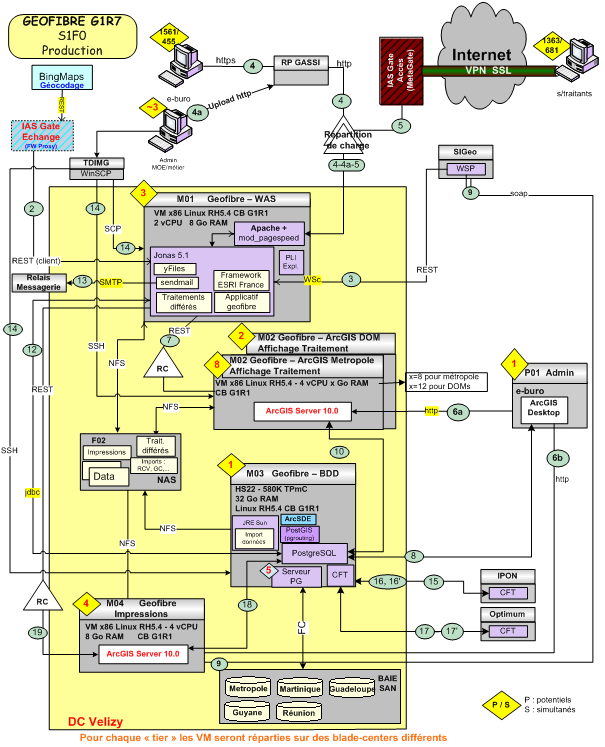
\includegraphics[width=16cm]{images/archtech.png}
  }
\end{figure}

\end{document}
